% Copyright 2008 Markus Kohm
% 
% This work may be distributed and/or modified under the
% conditions of the LaTeX Project Public License, either version 1.3
% of this license or (at your option) any later version.
% The latest version of this license is in
% http://www.latex-project.org/lppl.txt
% and version 1.3 or later is part of all distributions of LaTeX
% version 2005/12/01 or later.
% 
% This work has the LPPL maintenance status `maintained'.
% 
% The Current Maintainer of this work is Markus Kohm.
% 
% This work consists of this file only.
%-----------------------------------------------------------------------
\documentclass[parskip=half, a4paper]{scrartcl}

\usepackage[ngerman,english]{babel}
\usepackage{helvet}
\usepackage{graphicx}


%http://de.wikibooks.org/wiki/LaTeX-W%C3%B6rterbuch:_fontfamily
\renewcommand{\familydefault}{\sfdefault}
\fontfamily{phv}\selectfont

\begin{document}

\title{Database System Project}
\subtitle{Hunger -- System requirement report}
\author{Chris\\
		Saulo \\
		Alexander Goscinski -- 7120309027}
\date{\today}
\maketitle

\section{Functional specification}
Our project is an implementation of an food delivery system accesible by
a webpage. 
\begin{figure}[h]
	\centering
		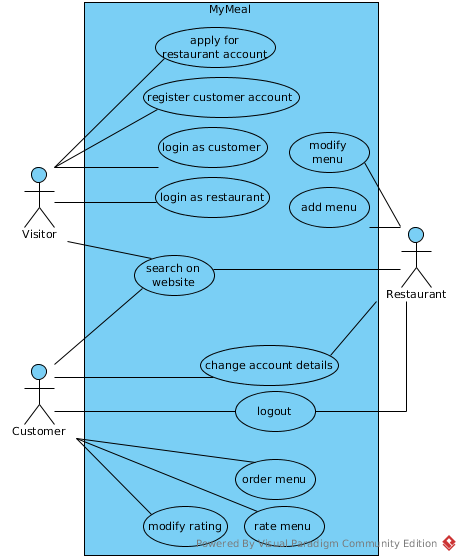
\includegraphics[scale=0.4]{UseCaseDiagramHunger.png}
	\caption{Use case diagram of our system.}
\end{figure}
Our system provides to any kind of the
service of searching for restaurants and food avaible for ordering. An user, who is not
logged in the system, can login as a user or
as a restaurant, register an user account and also apply for an restaurant account.
For now the application of a restaurant account will be processed similar to the
registration of an user account.

An user logged in an user account has the following possibilities: search
for restaurants or meals, cancel order, rating a menu after it was
devlivered, modify his/her rating his rating, modifying account details,
order menu, cancel order

An user logged in a restaurant account should be able to add, modify 
his/her menus as well as the account details, cancel and accept order
received from an registered user.

Optional goals: An application process for the restaurants, with 
approvement of an additional kind of user. In addition we would offer
an recommendation system for the user based on the users orders and 
ratings.

\section{Technical specification}
The Server will run on python and we use the Rest interface for communication
between front and back end. For the front end we use HTML, Javascript and CSS.
The database will run on MySQL.

\end{document}



